\documentclass{article}
\usepackage{amsmath}
\usepackage{amsfonts}
\usepackage{graphicx}
\usepackage{geometry}

\geometry{a4paper, margin=1in}

\begin{document}

\title{Resolução do Problema de Programação Linear Inteira usando Branch-and-Bound}
\author{João Victor Walcacer Giani\\ Professor: Warley Gramacho}
\date{22 de Outubro de 2024}
\maketitle

\section{Descrição do Problema de Programação Linear Inteira}

O problema escolhido é:

\begin{equation}
\text{Maximizar } Z = 3x_1 + 2x_2
\end{equation}

Sujeito a:

\begin{align}
2x_1 + x_2 & \leq 6 \quad (1) \\
x_1 + 2x_2 & \leq 5 \quad (2) \\
x_1, x_2 & \geq 0 \quad  \\
x_1, x_2 & \in \mathbb{Z} \quad 
\end{align}

Neste problema, buscamos maximizar a função objetivo \(Z\) com restrições de capacidade, onde \(x_1\) e \(x_2\) devem ser números inteiros não negativos.

\section{Modelo Relaxado de Programação Linear (PPL)}

Para obter o modelo relaxado, removemos a restrição de integralidade, resultando no seguinte problema:

\begin{align}
\text{Maximizar } Z = 3x_1 + 2x_2 \\
\text{sujeito a:} \\
2x_1 + x_2 & \leq 6 \\
x_1 + 2x_2 & \leq 5 \\
x_1, x_2 & \geq 0
\end{align}

\section{Resolução do Problema Relaxado}

Usamos o método gráfico para resolver o problema relaxado.

\subsection{Determinando os Vértices das Restrições}

A primeira restrição \(2x_1 + x_2 = 6\) intercepta os eixos em:
\begin{itemize}
    \item Intercepto no eixo \(x_1\): \(x_1 = 3\) (quando \(x_2 = 0\))
    \item Intercepto no eixo \(x_2\): \(x_2 = 6\) (quando \(x_1 = 0\))
\end{itemize}

A segunda restrição \(x_1 + 2x_2 = 5\) intercepta os eixos em:
\begin{itemize}
    \item Intercepto no eixo \(x_1\): \(x_1 = 5\) (quando \(x_2 = 0\))
    \item Intercepto no eixo \(x_2\): \(x_2 = 2.5\) (quando \(x_1 = 0\))
\end{itemize}

\subsection{Identificando a Região Viável}

A região viável é formada pela interseção das áreas sob as duas retas e acima dos eixos \(x\) e \(y\), representando a área onde todas as restrições são satisfeitas.

\subsection{Vértices da Região Viável}

Para encontrar os vértices da região viável, resolvemos o sistema de equações:

\begin{align}
2x_1 + x_2 & = 6 \\
x_1 + 2x_2 & = 5
\end{align}

Resolvendo o sistema:

Multiplicamos a segunda equação por 2 e subtraímos da primeira:

\begin{align}
4x_1 + 2x_2 & = 12 \\
-(x_1 + 2x_2) & = -5 \\
\hline
3x_1 & = 7 \\
x_1 & = \frac{7}{3} \approx 2.33
\end{align}

Substituindo o valor de \(x_1\) na primeira equação:

\begin{align}
2\left(\frac{7}{3}\right) + x_2 & = 6 \\
\frac{14}{3} + x_2 & = 6 \\
x_2 & = 6 - \frac{14}{3} = \frac{18}{3} - \frac{14}{3} = \frac{4}{3} \approx 1.33
\end{align}

Assim, temos um vértice: \( \left( \frac{7}{3}, \frac{4}{3} \right) \).

Os outros vértices da região viável são:
\begin{itemize}
    \item \(A(0, 0)\)
    \item \(B(3, 0)\)
    \item \(C(0, 2.5)\)
    \item \(D\left( \frac{7}{3}, \frac{4}{3} \right)\)
\end{itemize}

\section{Avaliação dos Vértices}

Agora, calculamos o valor da função objetivo \(Z\) em cada vértice:

\begin{itemize}
    \item Para \(A(0, 0)\):
    \[
    Z = 3(0) + 2(0) = 0
    \]

    \item Para \(B(3, 0)\):
    \[
    Z = 3(3) + 2(0) = 9
    \]

    \item Para \(C(0, 2.5)\):
    \[
    Z = 3(0) + 2(2.5) = 5
    \]

    \item Para \(D\left( \frac{7}{3}, \frac{4}{3} \right)\):
    \[
    Z = 3\left( \frac{7}{3} \right) + 2\left( \frac{4}{3} \right) = 7 + \frac{8}{3} = \frac{21}{3} + \frac{8}{3} = \frac{29}{3} \approx 9.67
    \]
\end{itemize}

O valor máximo da função objetivo para o modelo relaxado ocorre no ponto \(D\left( \frac{7}{3}, \frac{4}{3} \right)\) com \(Z \approx 9.67\).
\section{Bifurcações na Árvore de Branch-and-Bound}

A solução relaxada \(D\left(\frac{7}{3}, \frac{4}{3}\right)\) não é inteira, pois \(x_1\) e \(x_2\) assumem valores fracionários. Portanto, iniciamos o processo de bifurcação.

\section{Bifurcações no Problema de Programação Inteira}

\subsection{Primeira Bifurcação}

Escolhemos bifurcar em \(x_1\):
\begin{itemize}
    \item \textbf{Caso 1}: \(x_1 \leq 2\)
    \item \textbf{Caso 2}: \(x_1 \geq 3\)
\end{itemize}

\subsection{Resolvendo o Caso 1: \(x_1 \leq 2\)}

Considerando o problema original com a nova restrição:

\textbf{Função Objetivo:}
\[
Z = 3x_1 + 2x_2
\]

\textbf{Restrições:}
\[
\begin{aligned}
2x_1 + x_2 &\leq 6 \\
x_1 + 2x_2 &\leq 5 \\
x_1 &\leq 2 \\
x_1, x_2 &\geq 0 \quad (\text{inteiros})
\end{aligned}
\]

\subsection{ Método Gráfico para o Caso 1}

1. \textbf{Gráfico das Restrições}:
   \begin{itemize}
       \item \textbf{Reta 1}: \(2x_1 + x_2 = 6\)
       \item \textbf{Reta 2}: \(x_1 + 2x_2 = 5\)
       \item \textbf{Reta 3}: \(x_1 = 2\)
   \end{itemize}

2. \textbf{Pontos de Interseção}:
   - Interseção das retas \(2x_1 + x_2 = 6\) e \(x_1 + 2x_2 = 5\):
     \begin{itemize}
         \item Resolvendo o sistema:
         \[
         x_2 = 6 - 2x_1
         \]
         Substituindo na segunda restrição:
         \[
         x_1 + 2(6 - 2x_1) = 5 \implies x_1 + 12 - 4x_1 = 5 \implies -3x_1 = -7 \implies x_1 = \frac{7}{3} \approx 2.33
         \]
         \item Substituindo \(x_1\) na primeira equação para encontrar \(x_2\):
         \[
         x_2 = 6 - 2\left(\frac{7}{3}\right) = 6 - \frac{14}{3} = \frac{18}{3} - \frac{14}{3} = \frac{4}{3} \approx 1.33
         \]
     \end{itemize}

Os pontos a serem avaliados incluem:
   \begin{itemize}
       \item (0, 0)
       \item (0, 6)
       \item \(\left(\frac{7}{3}, \frac{4}{3}\right)\) (ponto de interseção)
       \item (2, 2) (ponto da nova restrição)
   \end{itemize}

3. \textbf{Solução do Caso 1}:
   Avaliando \(Z\) nos pontos relevantes:
   \begin{itemize}
       \item Para (0, 0): \(Z = 3(0) + 2(0) = 0\)
       \item Para (2, 2): \(Z = 3(2) + 2(2) = 6 + 4 = 10\)
       \item Para \(\left(\frac{7}{3}, \frac{4}{3}\right)\): \(Z = 3\left(\frac{7}{3}\right) + 2\left(\frac{4}{3}\right) = 7 + \frac{8}{3} \approx 11.67\) (não viável, pois \(x_1 > 2\))
   \end{itemize}

Assim, a melhor solução para o Caso 1 é:
\begin{itemize}
    \item \(x_1 = 2\)
    \item \(x_2 = 2\)
    \item \textbf{Valor de \(Z\)}: \(Z = 10\)
\end{itemize}

\subsection{Poda do Caso 1}

Como encontramos uma solução viável, não há poda nesse caso.

\subsection{ Resolvendo o Caso 2: \(x_1 \geq 3\)}

Agora, consideramos o problema original com a nova restrição:

\textbf{Função Objetivo:}
\[
Z = 3x_1 + 2x_2
\]

\textbf{Restrições:}
\[
\begin{aligned}
2x_1 + x_2 &\leq 6 \\
x_1 + 2x_2 &\leq 5 \\
x_1 &\geq 3 \\
x_1, x_2 &\geq 0 \quad (\text{inteiros})
\end{aligned}
\]

\subsection{ Método Gráfico para o Caso 2}

1. \textbf{Gráfico das Restrições}:
   \begin{itemize}
       \item \textbf{Reta 1}: \(2x_1 + x_2 = 6\)
       \item \textbf{Reta 2}: \(x_1 + 2x_2 = 5\)
       \item \textbf{Reta 3}: \(x_1 = 3\)
   \end{itemize}

2. \textbf{Pontos de Interseção}:
   - A interseção das retas \(2x_1 + x_2 = 6\) e \(x_1 + 2x_2 = 5\) é o mesmo ponto encontrado anteriormente:
     \[
     \left(\frac{7}{3}, \frac{4}{3}\right)
     \]

3. \textbf{Solução do Caso 2}:
   Avaliando \(Z\) nos pontos relevantes:
   \begin{itemize}
       \item Para (3, 0): \(Z = 3(3) + 2(0) = 9\)
       \item Para (3, 1): \(Z = 3(3) + 2(1) = 9 + 2 = 11\)
       \item Para (3, 2): \(Z = 3(3) + 2(2) = 9 + 4 = 13\) (não viável, pois \(x_2 > 2\))
   \end{itemize}

Assim, a melhor solução para o Caso 2 é:
\begin{itemize}
    \item \(x_1 = 3\)
    \item \(x_2 = 0\)
    \item \textbf{Valor de \(Z\)}: \(Z = 9\)
\end{itemize}

\subsection{Poda do Caso 2}

Como a solução encontrada no Caso 2 (\(Z = 9\)) é menor que a solução do Caso 1 (\(Z = 10\)), podemos podar essa bifurcação.

\subsection{Resumo das Soluções}

- \textbf{Caso 1}: \(x_1 = 2\), \(x_2 = 2\), \(Z = 10\)
- \textbf{Caso 2}: \(x_1 = 3\), \(x_2 = 0\), \(Z = 9\) (poda)

Como a solução \(Z = 10\) é maior do que a solução da relaxação original (\(Z \approx 9.67\)), continuamos o processo de branch-and-bound.


\subsection{ Verificando o Caso 2: \(x_1 \geq 3\)}

Substituindo \(x_1 = 3\) na função objetivo:

\begin{align}
2(3) + x_2 & \leq 6 \\
x_2 & \leq 0
\end{align}

A única solução inteira é \(x_2 = 0\).

Calculando \(Z\):

\[
Z = 3(3) + 2(0) = 9
\]

Como \(Z = 9\) é menor que a solução do Caso 1, não precisamos continuar com essa bifurcação.

\section{ Descrição e Justificativas}

\subsection{ Descrição do Problema e sua Formulação Matemática}

O problema de maximização consiste em encontrar os valores inteiros de \(x_1\) e \(x_2\) que maximizam a função objetivo \(Z = 3x_1 + 2x_2\) sujeita às restrições de capacidade e não negatividade. A solução deve atender às condições de integralidade.

\subsection{Solução da Relaxação Linear do Problema (PPL)}

A relaxação linear nos forneceu um valor ótimo de \(Z \approx 9.67\) em \(\left(\frac{7}{3}, \frac{4}{3}\right)\), que não atende às restrições de integralidade.

\subsection{Desenho da árvore do Branch-and-Bound com as bifurcações exploradas}

\begin{figure}
    \centering
    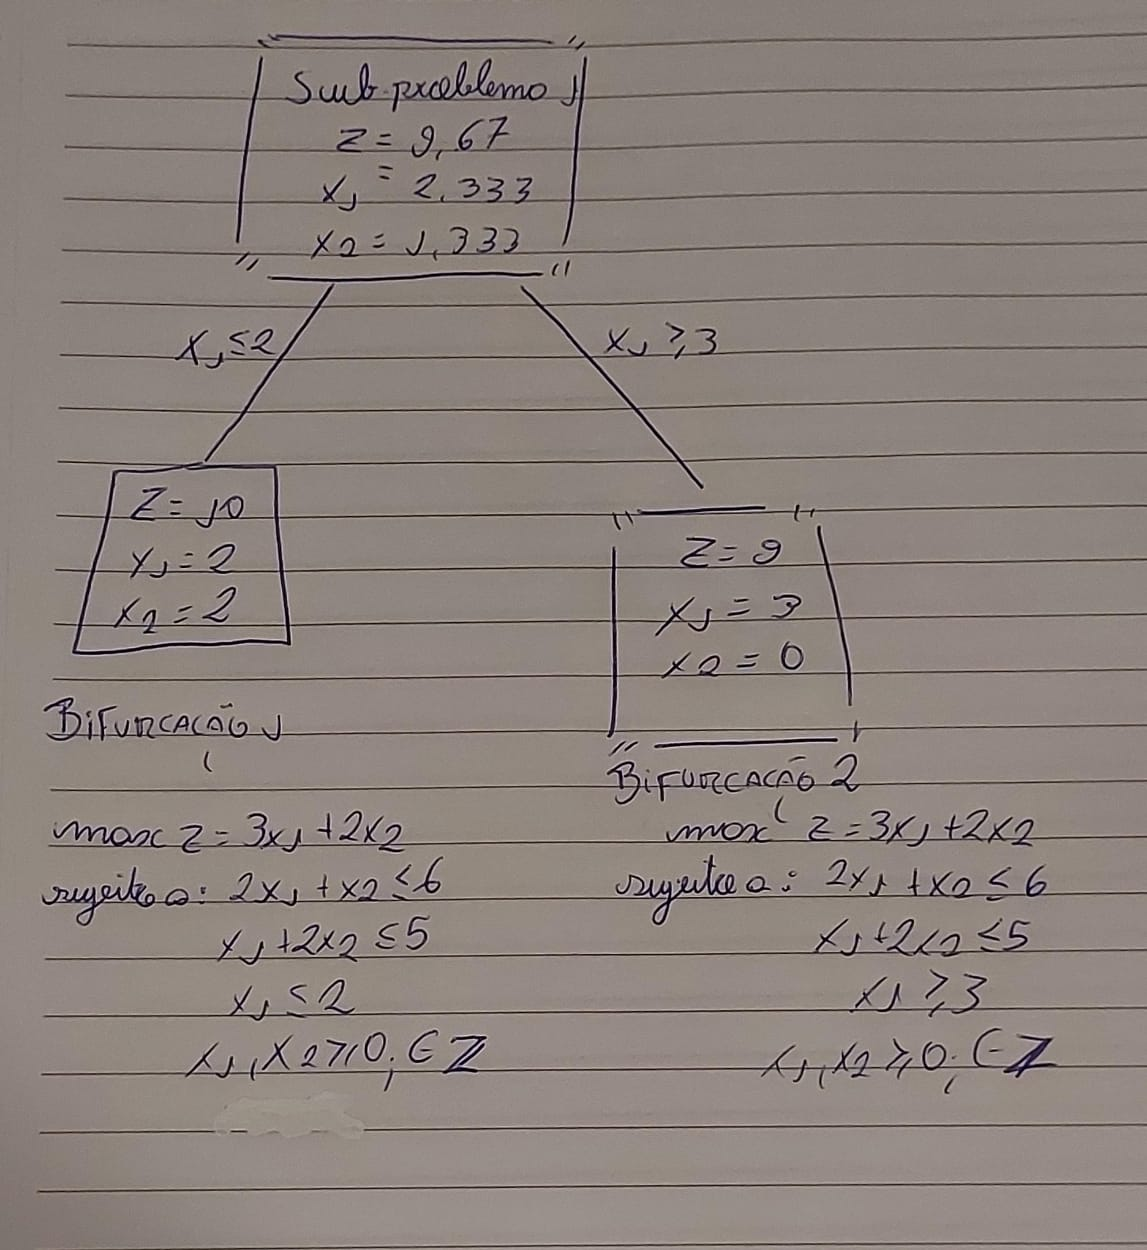
\includegraphics[width=0.5\linewidth]{arvore.jpg}
    \caption{Desenho da Árvore}
    \label{fig:enter-label}
\end{figure}

\newpage
\subsection{ Justificativas para as Podas Realizadas em Cada Nó da Árvore}

- **Caso 2** (\(x_1 \geq 3\)): A solução obtida \(Z = 9\) é inferior à melhor solução inteira encontrada até agora (\(Z = 10\)). Assim, podamos esse nó.
- **Caso 1** (\(x_1 \leq 2\)): O valor de \(Z = 10\) é a solução ótima encontrada e, portanto, mantivemos essa bifurcação.

\subsection{ A Solução Ótima Obtida ao Final da Execução do Algoritmo}

A solução ótima encontrada ao final da execução do algoritmo é:

\begin{align}
x_1 & = 2 \\
x_2 & = 2 \\
Z & = 10
\end{align}

\end{document}
